% ppo_heatmap_placeholder.tex
%
% Placeholder TikZ figure for §4 (Trainability).
% Renders an empty labelled 3x3 heatmap (kappa rows x beta cols) with a
% "Data pending (issue #360)" overlay. NO numerical values appear here.
% Replace once issue #360 completes the 4-seed PPO sweep over the 7-cell
% phase-diagram grid.
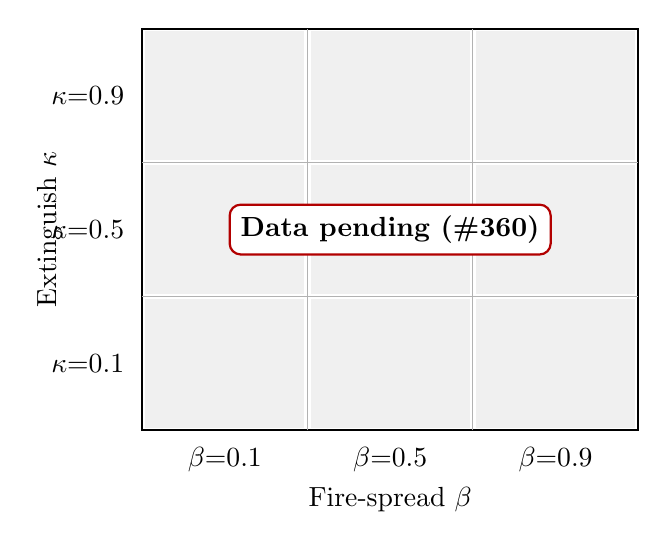
\begin{tikzpicture}[x=2.1cm,y=1.7cm]
  % Outer frame
  \draw[thick] (0,0) rectangle (3,3);
  % Grid lines
  \foreach \i in {1,2} {
    \draw[gray!60] (\i,0) -- (\i,3);
    \draw[gray!60] (0,\i) -- (3,\i);
  }
  % Empty cells (shaded light gray to signal "no data")
  \foreach \i in {0,1,2} {
    \foreach \j in {0,1,2} {
      \fill[gray!12] (\i+0.02,\j+0.02) rectangle (\i+0.98,\j+0.98);
    }
  }
  % Column labels (beta values)
  \node[below] at (0.5,-0.05) {$\beta{=}0.1$};
  \node[below] at (1.5,-0.05) {$\beta{=}0.5$};
  \node[below] at (2.5,-0.05) {$\beta{=}0.9$};
  % Row labels (kappa values), bottom-to-top
  \node[left] at (-0.05,0.5) {$\kappa{=}0.1$};
  \node[left] at (-0.05,1.5) {$\kappa{=}0.5$};
  \node[left] at (-0.05,2.5) {$\kappa{=}0.9$};
  % Axis titles
  \node[below=0.6cm] at (1.5,0) {Fire-spread $\beta$};
  \node[rotate=90,above=0.9cm] at (0,1.5) {Extinguish $\kappa$};
  % "Data pending" overlay
  \node[fill=white,draw=red!70!black,thick,rounded corners,inner sep=4pt,
        font=\bfseries] at (1.5,1.5) {Data pending (\#360)};
\end{tikzpicture}
